\chapter{Digital Circuits}

\begin{figure}[h!]
\centering
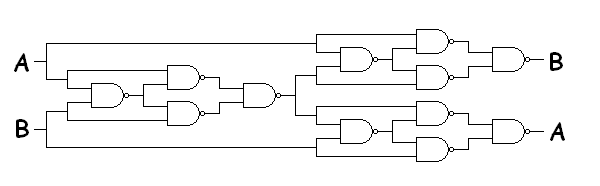
\includegraphics[width=6in]{d-ckt/d-ckt.png}
\caption{Typical digital circuit
of NAND gates.}
\label{fig-d-ckt}
\end{figure}

{\bf Digital (logic) gate:} node with
$na$ input ports and $nx$ output ports
which represents a function

\beq
f:\bool^{na}\rarrow \bool^{nx}
\;.
\label{eq-f-gate}
\eeq

Suppose

$a^{na}=(a_i)_{i=0, 1,\dots, na-1}$ 
where $a_i\in \bool$,

$x^{nx}=(x_i)_{i=0, 1,\dots, nx-1}$ 
where $x_i\in \bool$. 

$f$ maps $a^{na}$ into $x^{nx}$.

{\bf Digital circuit (dcircuit)} = circuit of digital gates.

\begin{figure}[h!]
\centering
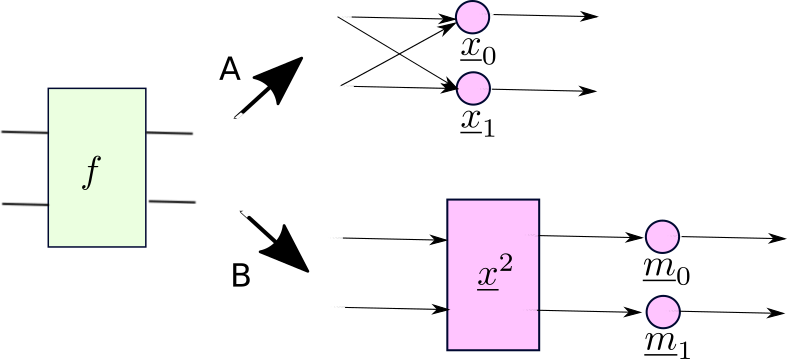
\includegraphics[width=3in]{d-ckt/d-ckt-2ops.png}
\caption{2 options
for mapping dcircuit node with
multiple output ports into bnet.}
\label{fig-d-ckt-2ops}
\end{figure}

\hrule\noindent
{\bf Mapping any
dcircuit to a bnet (Option A-
See Fig.\ref{fig-d-ckt-2ops})):}
\begin{enumerate}
\item
Replace every dcircuit  gate 
described by Eq.(\ref{eq-f-gate})
by
$nx$ bnet nodes $\rvx_i$
for $i=0, 1, \ldots, nx-1$
such that

\beq
P(x_i|a^{na})=\delta(x_i, f_i(a^{na}))
\eeq
\item
Replace
all connectors of the dcircuit
by arrows 
pointing in the direction
of the bit flow.

\end{enumerate}

\hrule\noindent
{\bf Mapping any
dcircuit to a bnet (Option B-
See Fig.\ref{fig-d-ckt-2ops})):}
\begin{enumerate}
\item
Replace every dcircuit  gate 
described by Eq.(\ref{eq-f-gate})
with
one bnet node called $\rvx^{nx}$
and, if $nx>0$, 
$nx$ ``marginalizer nodes" $\rvm_i$
for $i=0, 1, \ldots, nx-1$, such that

\beq\color{blue}
P(x^{nx}|a^{na})=
\delta(x^{nx}, f(a^{na}))
\;,
\eeq
and
\beq\color{blue}
P(m_i|x^{nx})=
\delta(m_i, x_i))
\;.
\eeq


\item
Replace
all connectors of the dcircuit
by arrows 
pointing in the direction
of the bit flow.



\end{enumerate}
\hrule 
Options A and B don't work
for digital circuits 
with feedback loops 
such as flip-flops.